%!TEX ROOT = ../manual_CZ.tex


Dostává se Vám do ruky uživatelský manuál modelu \smod. Celý název modelu je: Simulační Model Povrchového Odtoku a Erozního Procesu. Tento model lze využít pro výpočet hydrologicko erozních procesů na jednotlivých pozemcích nebo na malých povodích. Výstupy z modelu jsou primárně určeny pro stanovení odtokových poměrů v ploše povodí a parametrů opatření pro snížení odtoku z povodí a erozního ohrožení zemědělské půdy. Model lze využít při navrhování komplexnějších soustav sběrných a odváděcích prvků nebo suchých nádrží a polderů. Jeho využití předpokládají jak současné metodiky, tak i technické normy a doporučené standardy.
Z hlediska kategorizace se jedná o fyzikálně založený plně distribuovaný dvourozměrný epizodní model. 
% 
Nově zavedené prostorové řešení (2D), které nahradilo dřívější profilovou verzi modelu, umožňuje komplexní řešení a náhled na celou řešenou lokalitu a přesnější popis zpravidla heterogenní morfologie zemského povrchu. 
% 
Přechod modelu na 2D řešení umožňuje zejména větší dostupnost potřebných dat a zvyšující se kapacita výpočetní techniky. 
% 
% Přesto, že dvourozměrné řešení je z hlediska vstupních dat a vnitřních procesů složitější, nicméně benefity distribuovaného řešení převažují. 
% Dostupnost vstupních dat v podrobném rozlišení se zlepšuje, stejně tak jako se zvyšuje výpočetní kapacita výpočetní techniky.
% 
% 
Vývoj modelu je podporován z veřejných prostředků a podílejí se na něm studenti a zaměstnanci Katedry hydromeliorací a krajinného inženýrství Fakulty stavební ČVUT v Praze.
Pro snazší orientaci je manuál rozdělen na dvou hlavních částí. 
% 
V první části jsou uvedeny zvolené výpočetní vztahy pro popis povrchového odtoku. 
% 
Druhá část je věnována popisu instalace a použití modelu v prostředí ArcGIS. Dále jsou zde podrobně popsána vstupní a výstupní data a stručně popsán tok programu. 
% Ve třetí části jsou ukázány výsledky z řečení konkrétní lokality.
Případné aktualizace, vzorová data, ukázky využití a další informace o modelu \smod jsou průběžně poskytovány na webových stránkách (\href{http://storm.fsv.cvut.cz/cinnost-katedry/volne-stazitelne-vysledky/smoderp/?lang=cz}{storm.fsv.cvut.cz/cinnost-katedry/volne-stazitelne-vysledky/smoderp/}).


\subsection*{Hydrologické modelování}\addcontentsline{toc}{subsection}{Hydrologické modelování}
Hydrologické modelování s využitím geografických informačních sytému (GIS) je oblast vyvíjející se od konce 70. let. Hydrologické modelu využívaly (a využívají) technologii operací s geodaty a databázemi, které GIS umožňuje. Přesto jsou některé topologické operace pro hydrologické modely specifické (např. definice rozvodnice povodí, lokalizace/odstranění bezodtokových míst)~\citep{devantier1993}. V zásadě se rozvíjeli modelu povrchového odtoku založené na pravidelném rastru, nepravidelné trojúhelníkové síťi (TIN) nebo na vrstevnisích (contour-based)~\citep{devantier1993}. Rovněž docházelo k vývoji celistvých~\footnote{povodí je rozděleno na sub-povodí která jsou řešena celistvě například metodou SCS křivek} nebo plně distribuovaných modelů~\citep{devantier1993}. S vývojem informační techniky docházelo k větší integraci GIS softwaru a hydrologických modelů. Na obrázku~\ref{fig:klasGISHyd} je ukázána klasifikace propojení GIS a hydrologických modelu na konci 90. let~\citep{sui1999}. Hydrologický model buďto pouze využívá některé funkcionality GIS softwaru (obrázek~\ref{fig:klasGISHyd}a). V opačném případě již vývojář GIS softwaru integruje do systému některé prvky hydrologických modelů (obrázek~\ref{fig:klasGISHyd}b). GIS software a hydrologické model si pouze vyměňují některá data (pomocí binárních nebo ascii souborů (obrázek~\ref{fig:klasGISHyd}c), nebo GIS software umožňuje ve svém prostření vložit uživatelem vytvořené skripty, která pak tvoří hydrologický model (obrázek~\ref{fig:klasGISHyd}b)\footnote{Toto je případ modelu SMODERP2D pokud je spouštěn v prostředí ArcGIS}~\citep{sui1999}. Autoři studie se k těmto postupů staví kriticky. Jejich základní výhradou je, že struktury GIS software vytvářejí bariery pro popis hydrologických dějů, které mají jistá specifika. Konceptualizace pomocí vrstev ať už rastrových  nebo vektorových nemusí vyjadřovat heterogenitu hydrologických dějů nebo užití stochastických modelů. GIS softwary často umožňují pouze limitovanou prací časové proměnlivými ději~\citep{sui1999}.

\begin{figure}
  \centering
  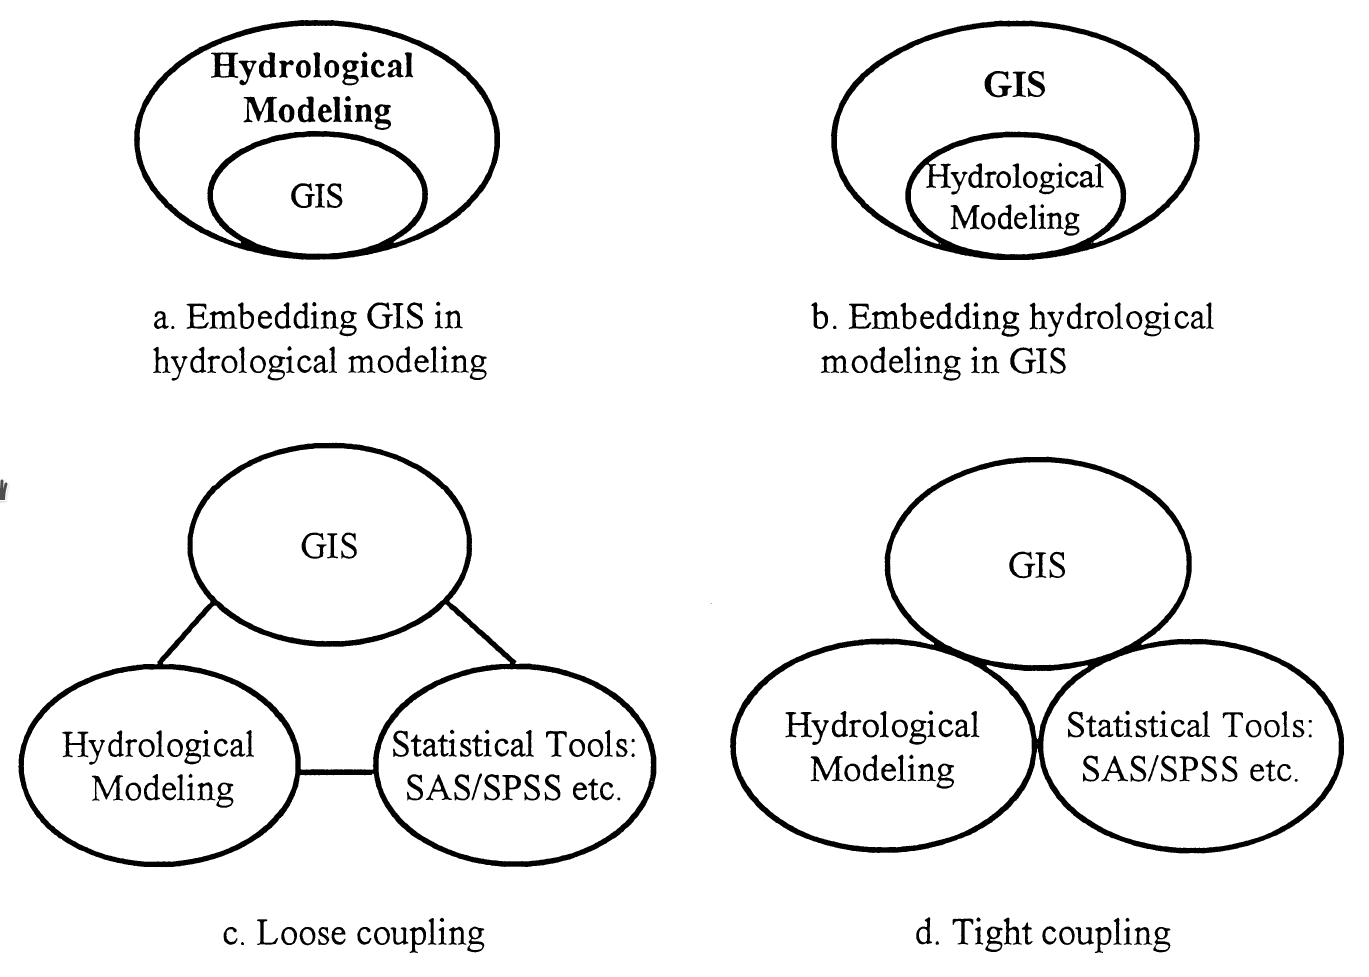
\includegraphics[width=\linewidth]{./img/klasifikaceGISHyd.png}
  \caption{Klasifikace integrace hydrologických modelu podle~\cite{sui1999}}
  \label{fig:klasGISHyd}
\end{figure}

Při popisu povrchového odtoku se nejčastěji využívá jedno ze zjednodušení Saint-Venantových (SV) rovnic ať už kinematickou nebo difuzní. 
\pozn{Diffuzni vlna zjednodušuje SV rovnice tím, že zanedbava člen konvekčního zrychlení (setrvacnost) (Chaudhry, 1993). pochopit a doplnit}
Příklad řešení povrchového odtoku pomocí kinematickou například: \cite{taylor1974} nebo \cite{goodrich1991}. V případě druhé studie bylo 2D řešení kinematické vlny řešeno pro jednotlivé trojúhelníky TIN sítě. Celkový odtok byl pak výpočtem 1D routingem odtoku z jednotlivých trojúhelníků TIN sítě. Kinematická vlna pro řešení povrchového odtoku je implementována například v modelu HEC-1~\citep{macarthur1993}. Jako příklad řešení povrchového odtoku pomocí difuzní vlny může být například~\cite{julien1995}, kde byla rovněž implementována prostorově distribuovaná srážka vhodná pro řešení bleskových povodí v aridních oblastech. V \cite{jain2004} bylo směrování odtoku definované pomocí jednosměrného algoritmu D8, samotný byla ale řešen pomocé difuzní vlny. Jako příklady softwaru, kde byla využita difuzní vlna k řešení povrchového odtoku je například: SHE~\cite{abbott1986_1, abbott1986_2}, CAS2D~\cite{julien1995}, WEPP~\citep{flanagan2010} nebo SWAT ~\citep{USDA}. V literatuře lze rovněž najít kritéria na základě kterých lze určit vhodnost obou řešení~\cite{singh1994, moramarco2002}

V modelech obecně je třeba dobře zvolit časovou a prostorovou diskretizaci.  U řešení povrchového odtoku byly zjištěny problémy s časovou diskretizací, kde docházelo k nestabilitám i při dodržení Courant–Friedrichs–Lewiho kritéria. To je způsobeno zejména malou hloubkou hladiny na povrchů vůči velikosti buňky rastru, drsnostnímu koeficientu nebo změně sklonu mezi sousedícími buňkamiA~\cite{zhang1989, esteves2000}. V \cite{molnar2000} byl studován vliv velikosti buňky rastru na výsledek modlu povrchového odtoku. Různá velikost buněk v rastru příliš neovlivňovala výsledné řešení pokud byla kalibrace provedena na rastru se stejně velkou buňkou. U řešení s větší buňkou bylo na povodí větší oblast, kde vznikl povrchový odtok a po kalibraci byla větší drsnost koryt hydrografické sítě.







